\documentclass[conference,twocolumn]{IEEEtran}

% Packages
\usepackage[utf8]{inputenc}
\usepackage[T1]{fontenc}
\usepackage{kotex}
\usepackage{amsmath,amssymb,amsfonts}
\usepackage{graphicx}
\usepackage{textcomp}
\usepackage{xcolor}
\usepackage{booktabs}
\usepackage{algorithm}
\usepackage{algorithmic}
\usepackage{multirow}
\usepackage{cite}
\usepackage{hyperref}
\usepackage{array}
\usepackage{subfig}

% Define colors
\definecolor{codegreen}{rgb}{0,0.6,0}
\definecolor{codegray}{rgb}{0.5,0.5,0.5}
\definecolor{codepurple}{rgb}{0.58,0,0.82}

\begin{document}

\title{CNN-LSTM 기반 베어링 잔여 수명 예측:\\고급 신호처리 기법 적용}

\author{
\IEEEauthorblockN{김진욱}
\IEEEauthorblockA{기계공학과\\
서울과학기술대학교\\
서울특별시, 대한민국\\
Email: jinwook@seoultech.ac.kr}
\and
\IEEEauthorblockN{서승일}
\IEEEauthorblockA{기계시스템디자인공학과\\
서울과학기술대학교\\
서울특별시, 대한민국\\
Email: seungil@seoultech.ac.kr}
}

\maketitle

\begin{abstract}
구름 베어링의 잔여 수명(RUL) 예측은 산업 기계의 효과적인 예측 정비 전략 수립에 필수적이다. 본 논문에서는 합성곱 신경망(CNN)과 장단기 메모리(LSTM) 네트워크를 결합한 하이브리드 딥러닝 기법과 고급 신호처리 기술을 통합한 베어링 RUL 예측 방법을 제안한다. 제안하는 방법론은 밴드패스 필터링(1000-5000Hz), 힐버트 변환 기반 포락선 분석, Daubechies-4(Db4) 웨이블릿 분해를 활용하여 원시 진동 신호로부터 의미 있는 열화 특징을 추출한다. 추출된 특징에는 제곱평균제곱근(RMS), 엔트로피 측정치, 웨이블릿 계수(D4\_RMS, D5\_RMS, D5\_Entropy)가 포함되어 베어링 열화 진행을 효과적으로 포착한다. 제안하는 CNN-LSTM 구조는 25.6kHz로 샘플링된 다채널 진동 데이터로부터 공간적, 시간적 패턴을 동시에 학습한다. KSPHM-KIMM 2025 베어링 수명 예측 챌린지 데이터셋에서 검증한 결과, 70개 참가팀 중 7위를 달성하였다. 실험 결과는 물리 기반 신호처리와 딥러닝의 결합이 다양한 운전 조건에서도 강건한 RUL 예측을 가능하게 함을 보여준다.
\end{abstract}

\begin{IEEEkeywords}
베어링 고장 진단, 잔여 수명 예측, CNN-LSTM, 웨이블릿 변환, 포락선 분석, 예측 정비
\end{IEEEkeywords}

\section{서론}

구름 베어링은 회전 기계에서 가장 중요한 구성 요소 중 하나이며, 예기치 않은 고장은 산업 시스템에서 심각한 경제적 손실, 안전 위험 및 계획되지 않은 가동 중단을 초래할 수 있다 \cite{lei2018machinery}. 산업 조사에 따르면 베어링 고장은 전체 회전 기계 고장의 약 40-50\%를 차지한다 \cite{randall2011rolling}. 따라서 베어링의 정확한 잔여 수명(RUL) 예측 방법 개발은 고장 예지 및 건전성 관리(PHM) 분야에서 핵심적인 연구 주제로 부상하였다.

전통적인 베어링 상태 모니터링 방식은 진동 신호에서 추출한 통계적 특징을 이용한 임계값 기반 방법에 의존한다 \cite{jardine2006review}. 이러한 방법은 해석이 용이하고 계산 효율이 높지만, 실제 운전 조건에서 베어링이 보이는 복잡한 비선형 열화 패턴을 포착하는 데 한계가 있다. 더욱이 베어링의 열화 과정은 하중 변화, 속도 변화, 환경 조건 등 다양한 요인의 영향을 받아 정확한 RUL 예측을 어렵게 만든다.

최근 딥러닝의 발전은 베어링 예지에 새로운 가능성을 열었다. 합성곱 신경망(CNN)은 원시 또는 최소 처리된 신호로부터 계층적 특징을 자동으로 추출하는 탁월한 능력을 보여주었다 \cite{zhang2017new}. 장단기 메모리(LSTM) 네트워크는 순차 데이터의 장기 시간 의존성을 포착하는 데 뛰어나 열화 궤적 모델링에 적합하다 \cite{zhao2017machine}. CNN-LSTM으로 알려진 이 두 구조의 결합은 양쪽의 장점을 모두 활용한다: CNN 계층은 신호 구간에서 공간적 특징을 추출하고 LSTM 계층은 베어링 수명 동안 이러한 특징의 시간적 변화를 모델링한다.

그러나 딥러닝을 원시 진동 신호에 직접 적용하면 잡음과 관련 없는 주파수 성분의 존재로 인해 최적의 결과를 얻지 못할 수 있다. 밴드패스 필터링, 포락선 분석, 웨이블릿 변환과 같은 신호처리 기법은 신호 대 잡음비를 향상시키고 베어링 열화에 더 민감한 특징을 추출할 수 있다 \cite{antoni2007fast}. 물리 기반 신호처리를 통한 도메인 지식과 데이터 기반 딥러닝 모델의 통합은 RUL 예측 정확도 향상을 위한 유망한 방향을 제시한다.

본 논문에서는 고급 신호처리 기법과 CNN-LSTM 딥러닝 구조를 결합한 포괄적인 베어링 RUL 예측 접근법을 제시한다. 주요 기여는 다음과 같다:

\begin{itemize}
    \item 베어링 고장 특징 추출에 최적화된 밴드패스 필터링(1000-5000Hz), 힐버트 변환 기반 포락선 분석, Db4 웨이블릿 분해를 포함하는 신호처리 파이프라인 개발
    \item 베어링 열화 진행을 효과적으로 포착하는 다중 웨이블릿 스케일(D4, D5)의 RMS와 엔트로피를 포함한 물리 기반 특징 추출
    \item 다채널 진동 데이터로부터 공간적, 시간적 패턴을 동시에 학습하는 CNN-LSTM 구조 설계
    \item KSPHM-KIMM 2025 베어링 수명 예측 챌린지에서 70개 참가팀 중 7위 달성을 통한 검증
\end{itemize}

본 논문의 구성은 다음과 같다. 2장에서는 베어링 고장 진단 및 RUL 예측에 관한 관련 연구를 검토한다. 3장에서는 신호처리 기법, 특징 추출, CNN-LSTM 모델 구조를 포함한 방법론을 설명한다. 4장에서는 실험 환경과 결과를 제시한다. 5장에서는 결론과 향후 연구 방향에 대해 논의한다.

\section{관련 연구}

\subsection{베어링 고장 진단 및 예지}

베어링 고장 진단은 진동 분석 기법을 활용하여 광범위하게 연구되어 왔다. 전통적인 접근법은 시간 영역 통계적 특징(평균, 분산, RMS, 첨도, 파고율)과 주파수 영역 특징(스펙트럼 에너지, 지배 주파수) 추출에 초점을 맞춘다 \cite{randall2011rolling}. 힐버트 변환에 기반한 포락선 분석 기법은 베어링 결함에 의해 발생하는 주기적 충격을 검출하는 데 특히 효과적이다 \cite{mccormick1998cyclostationarity}.

웨이블릿 변환은 진동 신호를 다른 스케일의 근사 및 상세 계수로 분해하는 다중 해상도 분석 기능을 제공한다. 이산 웨이블릿 변환(DWT)은 베어링 결함과 관련된 과도 이벤트를 포착하는 능력으로 인해 베어링 고장 진단에 널리 사용된다 \cite{kumar2013wavelet}. 다양한 웨이블릿 계열 중 Daubechies 웨이블릿, 특히 Db4는 베어링 진동 분석에 효과적인 것으로 입증되었다 \cite{toma2020bearing, nizwan2016wavelet}.

\subsection{딥러닝 기반 RUL 예측}

딥러닝 방법은 최근 베어링 RUL 예측에서 상당한 관심을 받고 있다. 합성곱 신경망은 원시 진동 신호나 시간-주파수 표현으로부터 직접 특징을 학습하는 데 적용되었다 \cite{li2018remaining}. LSTM 네트워크는 베어링 건전성 지표의 시간적 변화를 모델링하는 데 활용되었다 \cite{zhao2017machine}.

CNN과 LSTM을 결합한 하이브리드 구조는 유망한 결과를 보여주었다. CNN 계층은 자동 특징 추출기 역할을 하고 LSTM 계층은 추출된 특징의 시간 의존성을 포착한다 \cite{chen2020bearing}. RUL 예측에 가장 관련성 높은 시간 단계에 집중하기 위해 어텐션 메커니즘도 도입되었다 \cite{wang2020remaining}.

이러한 발전에도 불구하고 많은 딥러닝 접근법은 문제를 순수하게 데이터 기반으로 처리하여 도메인 지식에서 얻을 수 있는 귀중한 통찰을 놓칠 수 있다. 최근 연구는 예측 정확도와 일반화 성능 향상을 위해 물리 기반 특징과 딥러닝 모델의 통합의 중요성을 강조하고 있다 \cite{li2020deep}.

\section{방법론}

\subsection{데이터 설명}

KSPHM-KIMM 2025 베어링 수명 예측 챌린지는 구름 베어링의 가동부터 고장까지의 진동 데이터를 제공한다. 데이터셋은 8개의 학습 세트와 6개의 검증 세트로 구성되며, 각각은 정상 상태에서 고장까지의 완전한 열화 과정을 나타낸다.

각 데이터 샘플은 TDMS 형식으로 저장되며 다음을 포함한다:
\begin{itemize}
    \item 25,600Hz로 샘플링된 4채널 진동 신호(CH1-CH4)
    \item 낮은 샘플링 레이트의 운전 조건 데이터(토크, 온도)
    \item 각 수집 주기는 10분 간격으로 10초간의 데이터 측정
\end{itemize}

진동 데이터는 파일당 채널당 256,000개의 데이터 포인트를 포함한다(25,600Hz $\times$ 10초). 다채널 구성은 다양한 센서 위치에서 베어링 진동의 포괄적인 모니터링을 가능하게 한다.

% Figure placeholder
\begin{figure}[t]
\centering
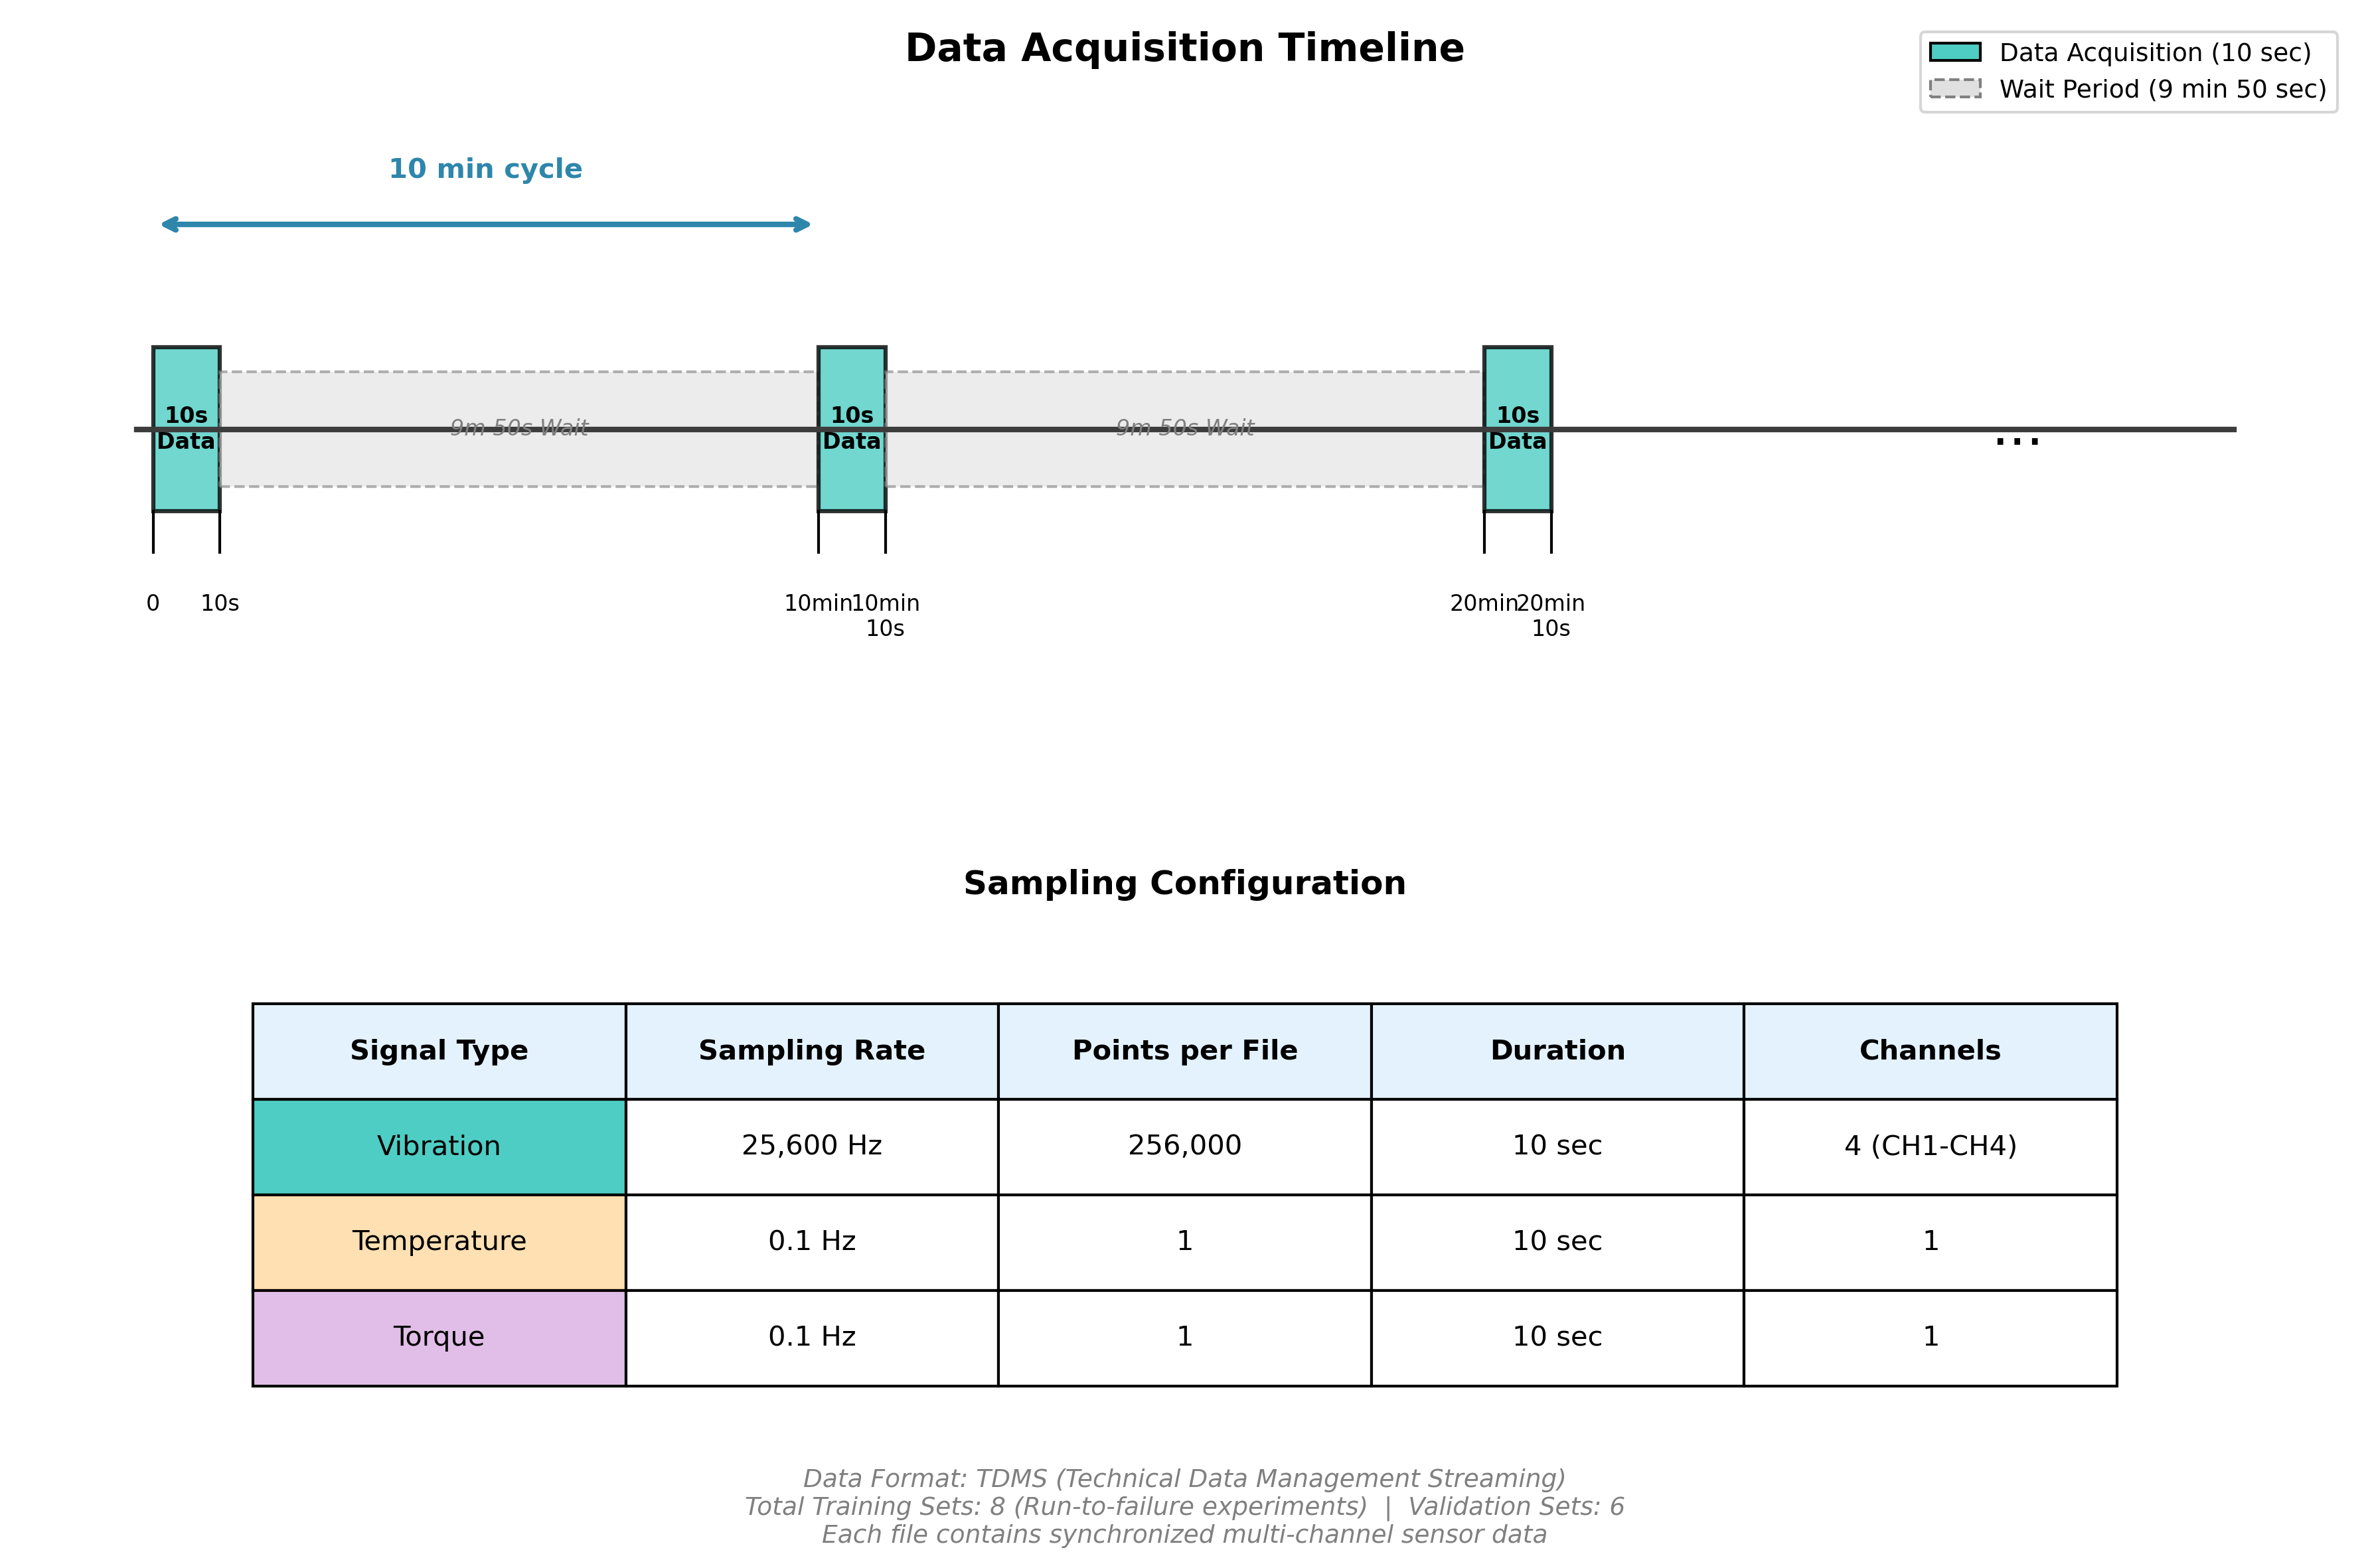
\includegraphics[width=0.9\columnwidth]{figures/data_acquisition.png}
\caption{데이터 수집 시스템 개요. 4채널 가속도계가 베어링 하우징에 설치되어 25.6kHz로 진동 신호를 측정한다.}
\label{fig:data_acquisition}
\end{figure}

\subsection{신호처리}

본 연구의 신호처리 파이프라인은 밴드패스 필터링, 포락선 분석, 웨이블릿 분해의 세 가지 주요 단계로 구성된다. 이러한 기법들은 잡음을 억제하면서 베어링 고장 관련 특징을 강화하도록 설계되었다.

% Figure placeholder
\begin{figure}[t]
\centering
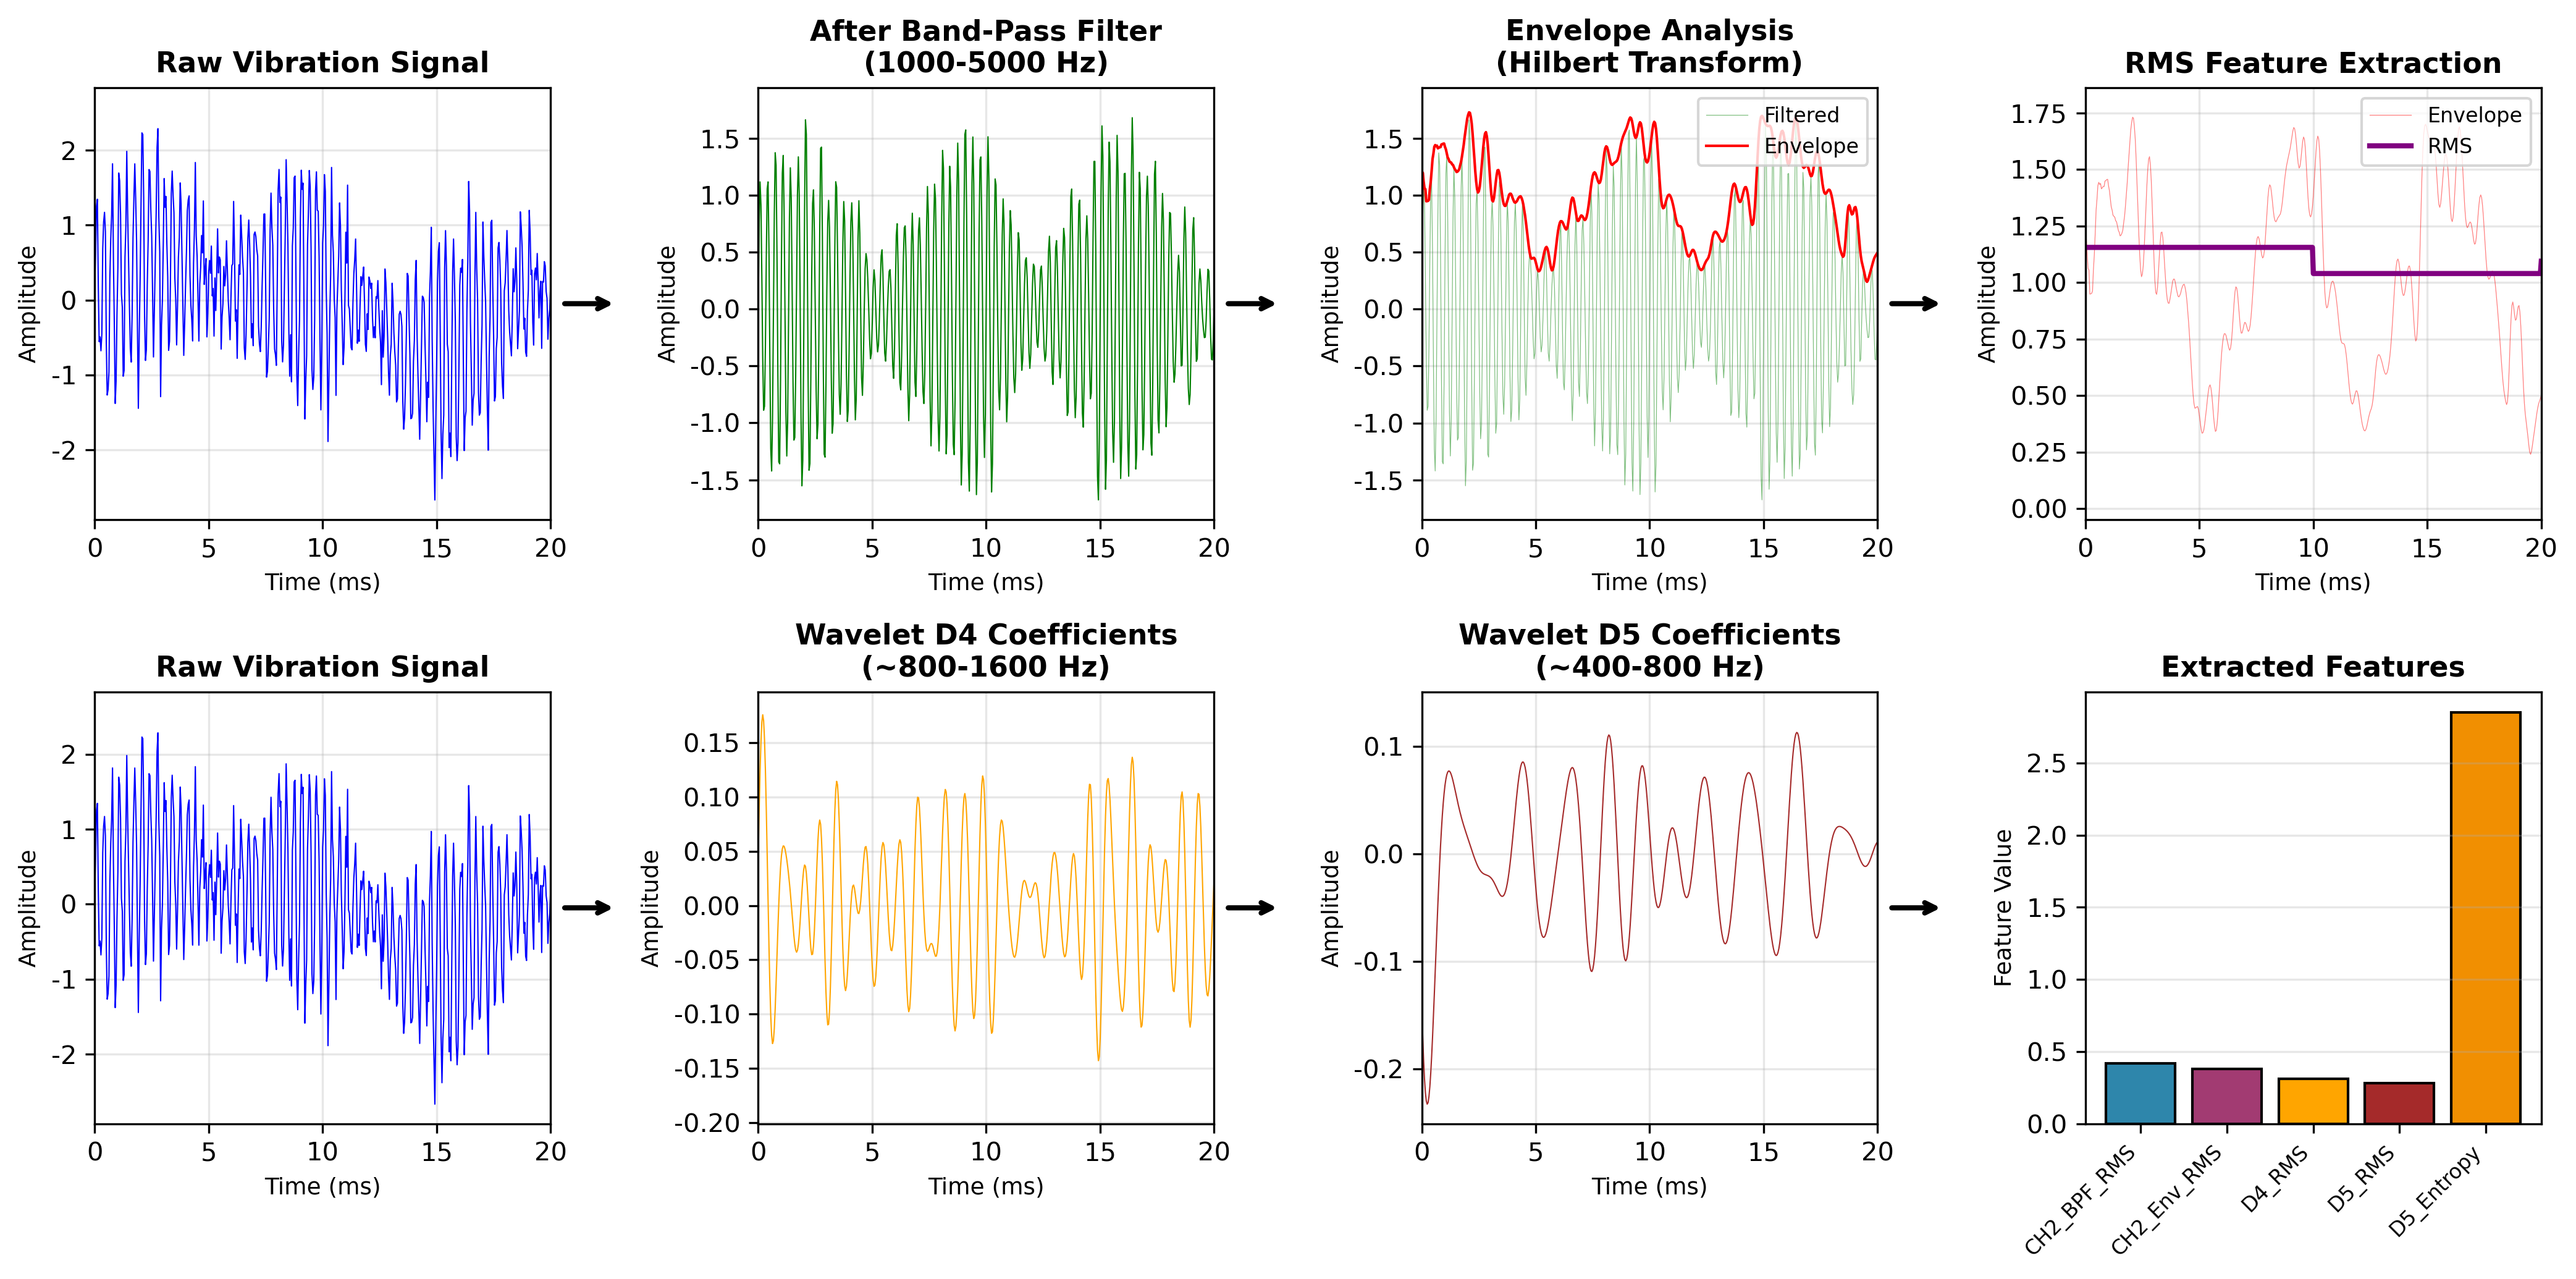
\includegraphics[width=0.9\columnwidth]{figures/signal_processing_concept.png}
\caption{신호처리 파이프라인 개념도. 원시 진동 신호가 밴드패스 필터링, 포락선 분석, 웨이블릿 분해를 거쳐 특징으로 변환된다.}
\label{fig:signal_processing}
\end{figure}

\subsubsection{밴드패스 필터}

진동 신호의 저주파 성분(1000Hz 이하)은 주로 구조적 진동과 외부 교란에 의해 지배되며, 고주파 성분(5000Hz 이상)은 잡음에 취약하다. 베어링 고장 주파수와 그 고조파 분석을 기반으로, 차단 주파수 1000Hz와 5000Hz를 갖는 4차 Butterworth 밴드패스 필터를 적용한다.

$n$차 Butterworth 밴드패스 필터의 전달함수는 다음과 같다:
\begin{equation}
    H(s) = \frac{H_0 \cdot (\omega_0/Q)s}{s^2 + (\omega_0/Q)s + \omega_0^2}
\end{equation}
여기서 $\omega_0 = \sqrt{\omega_L \cdot \omega_H}$는 중심 주파수, $Q = \omega_0/(\omega_H - \omega_L)$는 품질 계수, $\omega_L$, $\omega_H$는 각각 하한 및 상한 차단 주파수이다.

Butterworth 필터는 통과대역에서 최대 평탄 크기 응답을 특징으로 한다:
\begin{equation}
    |H(j\omega)|^2 = \frac{1}{1 + \left(\frac{\omega}{\omega_c}\right)^{2n}}
\end{equation}
여기서 $n$은 필터 차수, $\omega_c$는 차단 주파수이다.

% Figure placeholder
\begin{figure}[t]
\centering
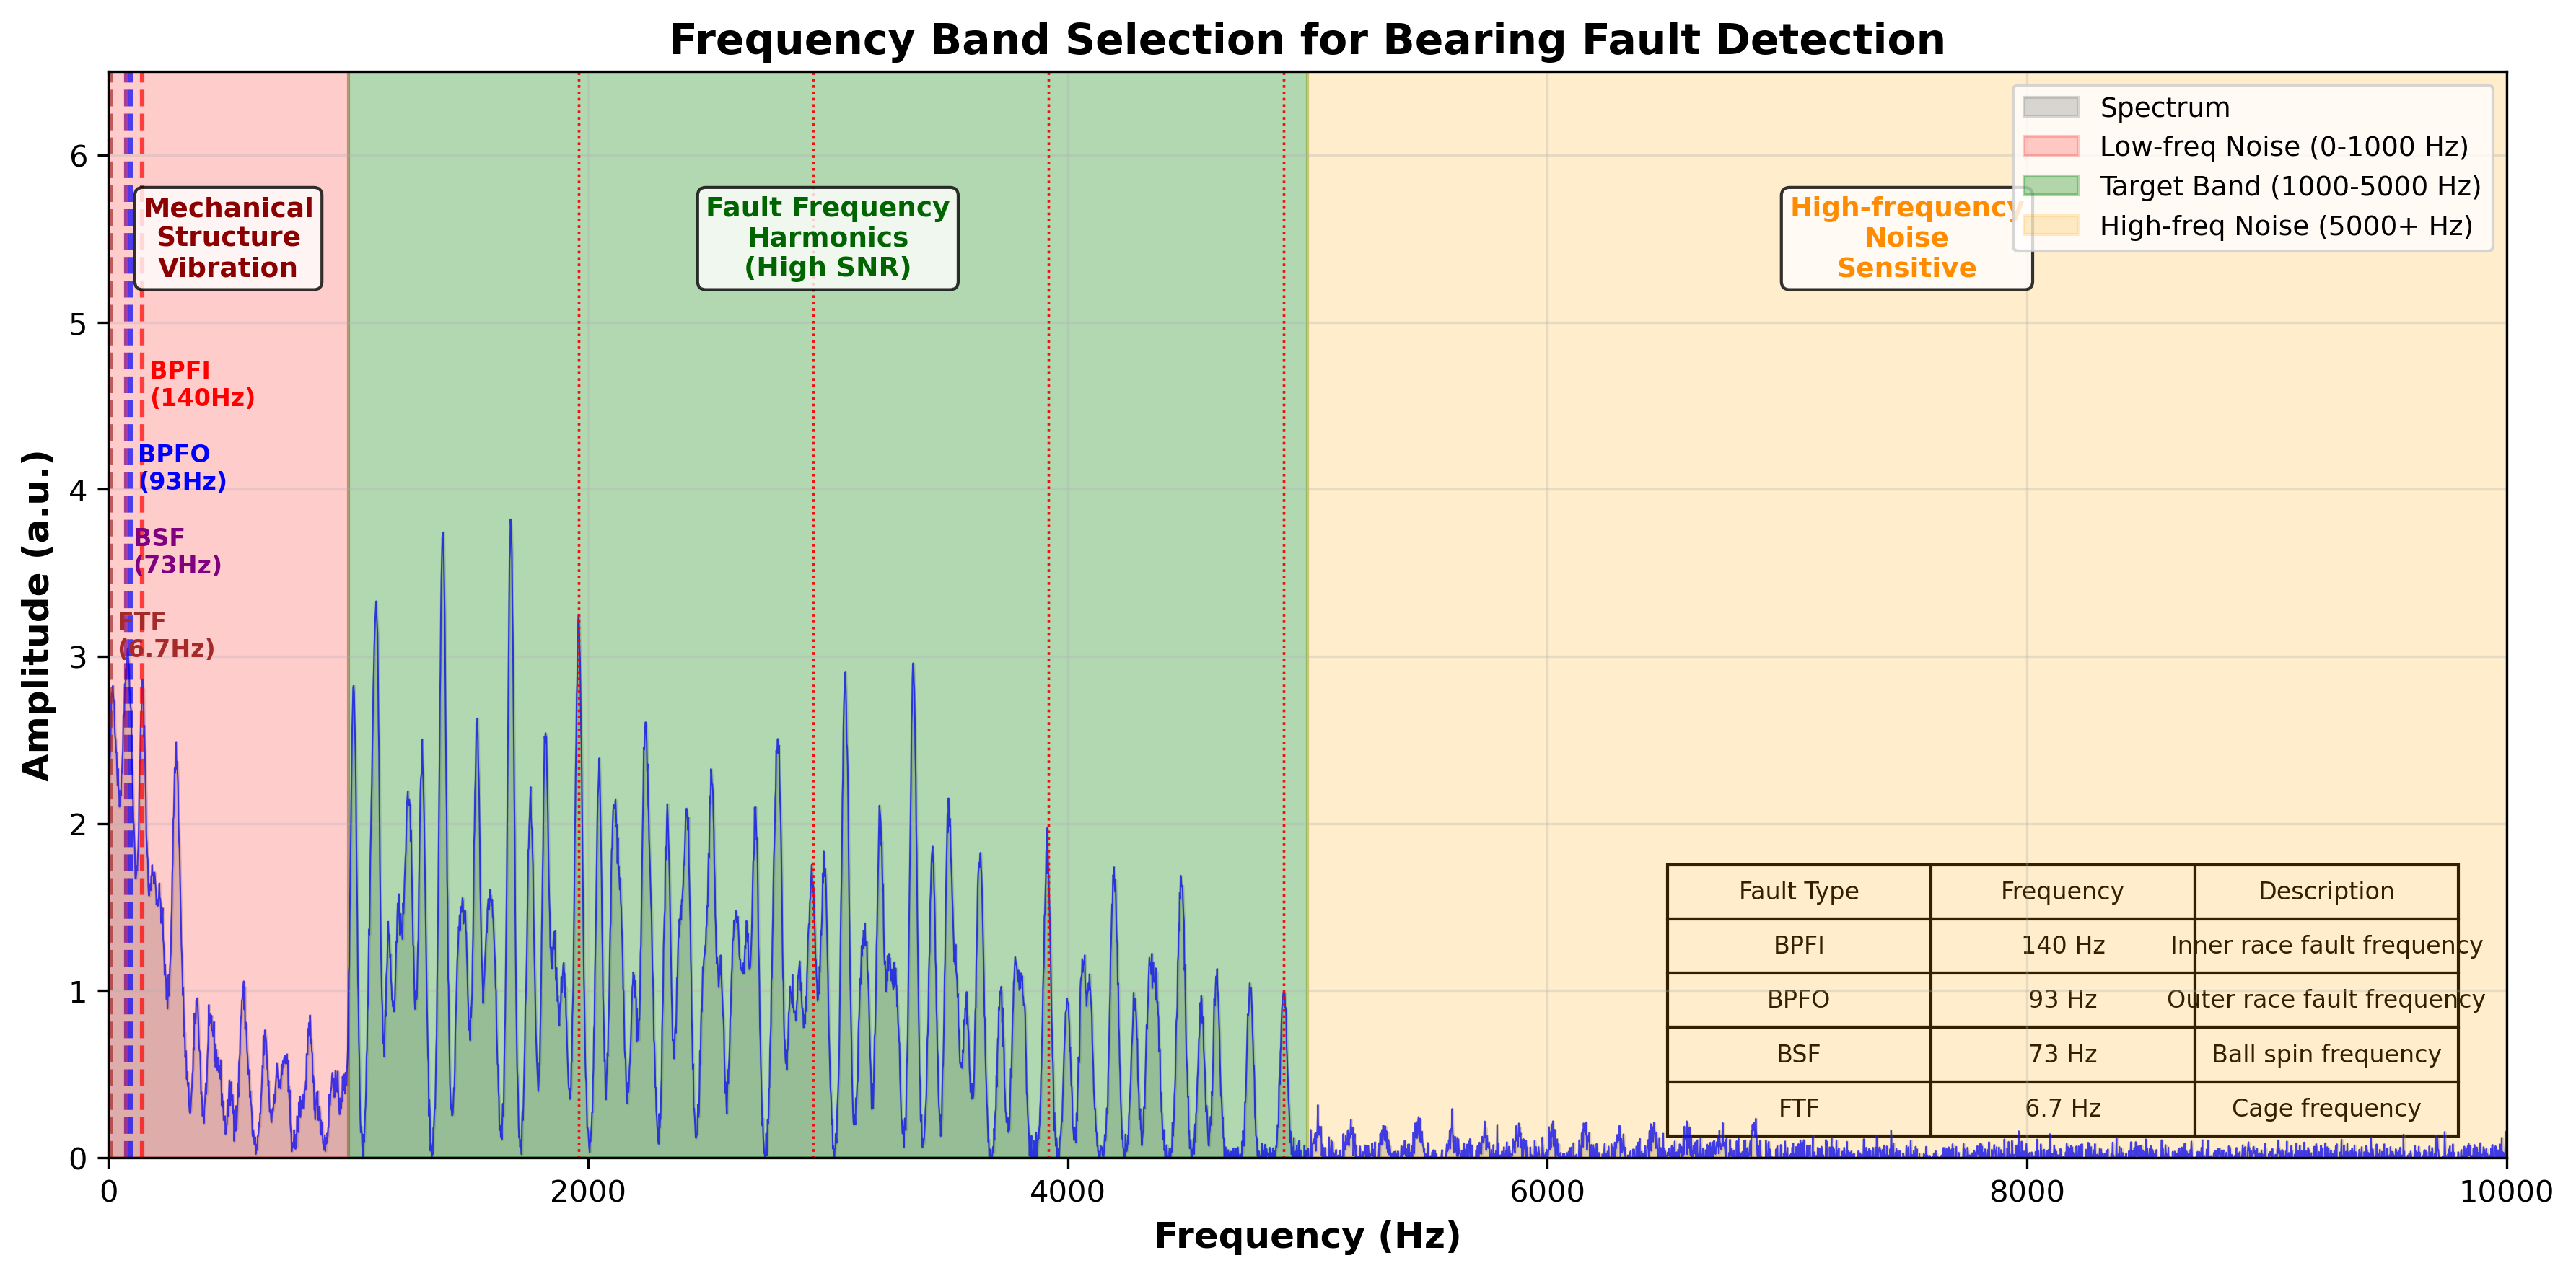
\includegraphics[width=0.9\columnwidth]{figures/frequency_band_selection.png}
\caption{주파수 대역 선정 근거. 1000-5000Hz 대역이 베어링 결함 특성 주파수를 가장 잘 포함하며 잡음 영향이 최소화된다.}
\label{fig:frequency_band}
\end{figure}

\subsubsection{포락선 분석}

힐버트 변환에 기반한 포락선 분석은 진동 신호의 진폭 변조 패턴을 추출하는 데 사용된다. 베어링 결함이 발생하면 구름 요소가 결함을 지나갈 때마다 주기적인 충격이 발생한다. 이러한 충격은 베어링과 하우징의 공진 주파수를 여기시켜 진폭 변조 신호를 생성한다.

신호 $x(t)$의 힐버트 변환은 다음과 같이 정의된다:
\begin{equation}
    \hat{x}(t) = \mathcal{H}\{x(t)\} = \frac{1}{\pi} \int_{-\infty}^{\infty} \frac{x(\tau)}{t - \tau} d\tau
\end{equation}

해석 신호는 다음과 같이 구성된다:
\begin{equation}
    z(t) = x(t) + j\hat{x}(t)
\end{equation}

포락선(순시 진폭)은 다음과 같이 얻어진다:
\begin{equation}
    A(t) = |z(t)| = \sqrt{x^2(t) + \hat{x}^2(t)}
\end{equation}

이 포락선 신호는 베어링 결함으로 인한 변조 패턴을 포착하여, 신호가 잡음으로 오염되어 있더라도 고장 특성 주파수의 검출을 가능하게 한다.

\subsubsection{웨이블릿 변환}

이산 웨이블릿 변환(DWT)은 진동 신호의 다중 해상도 분석을 제공하며, 다른 스케일에서 근사 및 상세 계수로 분해한다. 본 연구에서는 시간과 주파수 국소화 사이의 좋은 균형으로 인해 베어링 진동 분석에 효과적인 것으로 알려진 Daubechies-4(Db4) 웨이블릿을 사용한다 \cite{kumar2013wavelet}.

신호 $x(t)$의 DWT는 다음과 같이 계산된다:
\begin{equation}
    W_{\psi}(j, k) = \frac{1}{\sqrt{2^j}} \int_{-\infty}^{\infty} x(t) \psi^*\left(\frac{t - 2^j k}{2^j}\right) dt
\end{equation}
여기서 $\psi(t)$는 모 웨이블릿, $j$는 스케일 파라미터, $k$는 이동 파라미터이다.

분해 레벨 5에서 D1부터 D5까지의 상세 계수를 얻으며, 이는 각각 다른 주파수 대역에 해당한다. 분석 결과를 바탕으로 베어링 고장 특성과 가장 관련성이 높은 주파수 범위를 포착하는 D4와 D5 계수에 집중한다.

\subsection{특징 추출}

처리된 신호로부터 베어링 열화를 효과적으로 특성화하는 특징을 추출한다:

\subsubsection{제곱평균제곱근(RMS)}

RMS는 신호 에너지와 진동 진폭의 기본적인 지표이다:
\begin{equation}
    RMS = \sqrt{\frac{1}{N} \sum_{i=1}^{N} x_i^2}
\end{equation}
여기서 $N$은 샘플 수, $x_i$는 신호 값이다.

RMS는 다음으로부터 계산된다:
\begin{itemize}
    \item 밴드패스 필터링된 신호(CH2\_1000-5000Hz\_BPF)
    \item 밴드패스 필터링된 신호의 포락선(CH2\_1000-5000Hz\_RMS\_Envelope)
    \item 웨이블릿 상세 계수(D4\_RMS, D5\_RMS)
\end{itemize}

\subsubsection{섀넌 엔트로피}

섀넌 엔트로피는 신호의 복잡성 또는 불규칙성을 정량화한다:
\begin{equation}
    H = -\sum_{i} p(x_i) \log_2 p(x_i)
\end{equation}
여기서 $p(x_i)$는 신호 값의 확률 밀도이다.

베어링 열화가 진행됨에 따라 진동 신호의 불규칙성과 복잡성이 증가하여 엔트로피가 증가한다. 64개 빈을 사용한 히스토그램 기반 확률 추정을 통해 웨이블릿 D5 계수로부터 D5\_Entropy를 계산한다.

\subsubsection{특징 요약}

각 샘플에 대한 최종 특징 집합은 다음으로 구성된다:
\begin{itemize}
    \item CH2\_1000-5000Hz\_BPF: 밴드패스 필터링된 CH2 신호의 RMS
    \item CH2\_1000-5000Hz\_RMS\_Envelope: 포락선 신호의 RMS
    \item D4\_RMS: D4 웨이블릿 계수의 RMS (전체 채널)
    \item D5\_RMS: D5 웨이블릿 계수의 RMS (전체 채널)
    \item D5\_Entropy: D5 웨이블릿 계수의 엔트로피 (전체 채널)
\end{itemize}

% Figure placeholder
\begin{figure}[t]
\centering
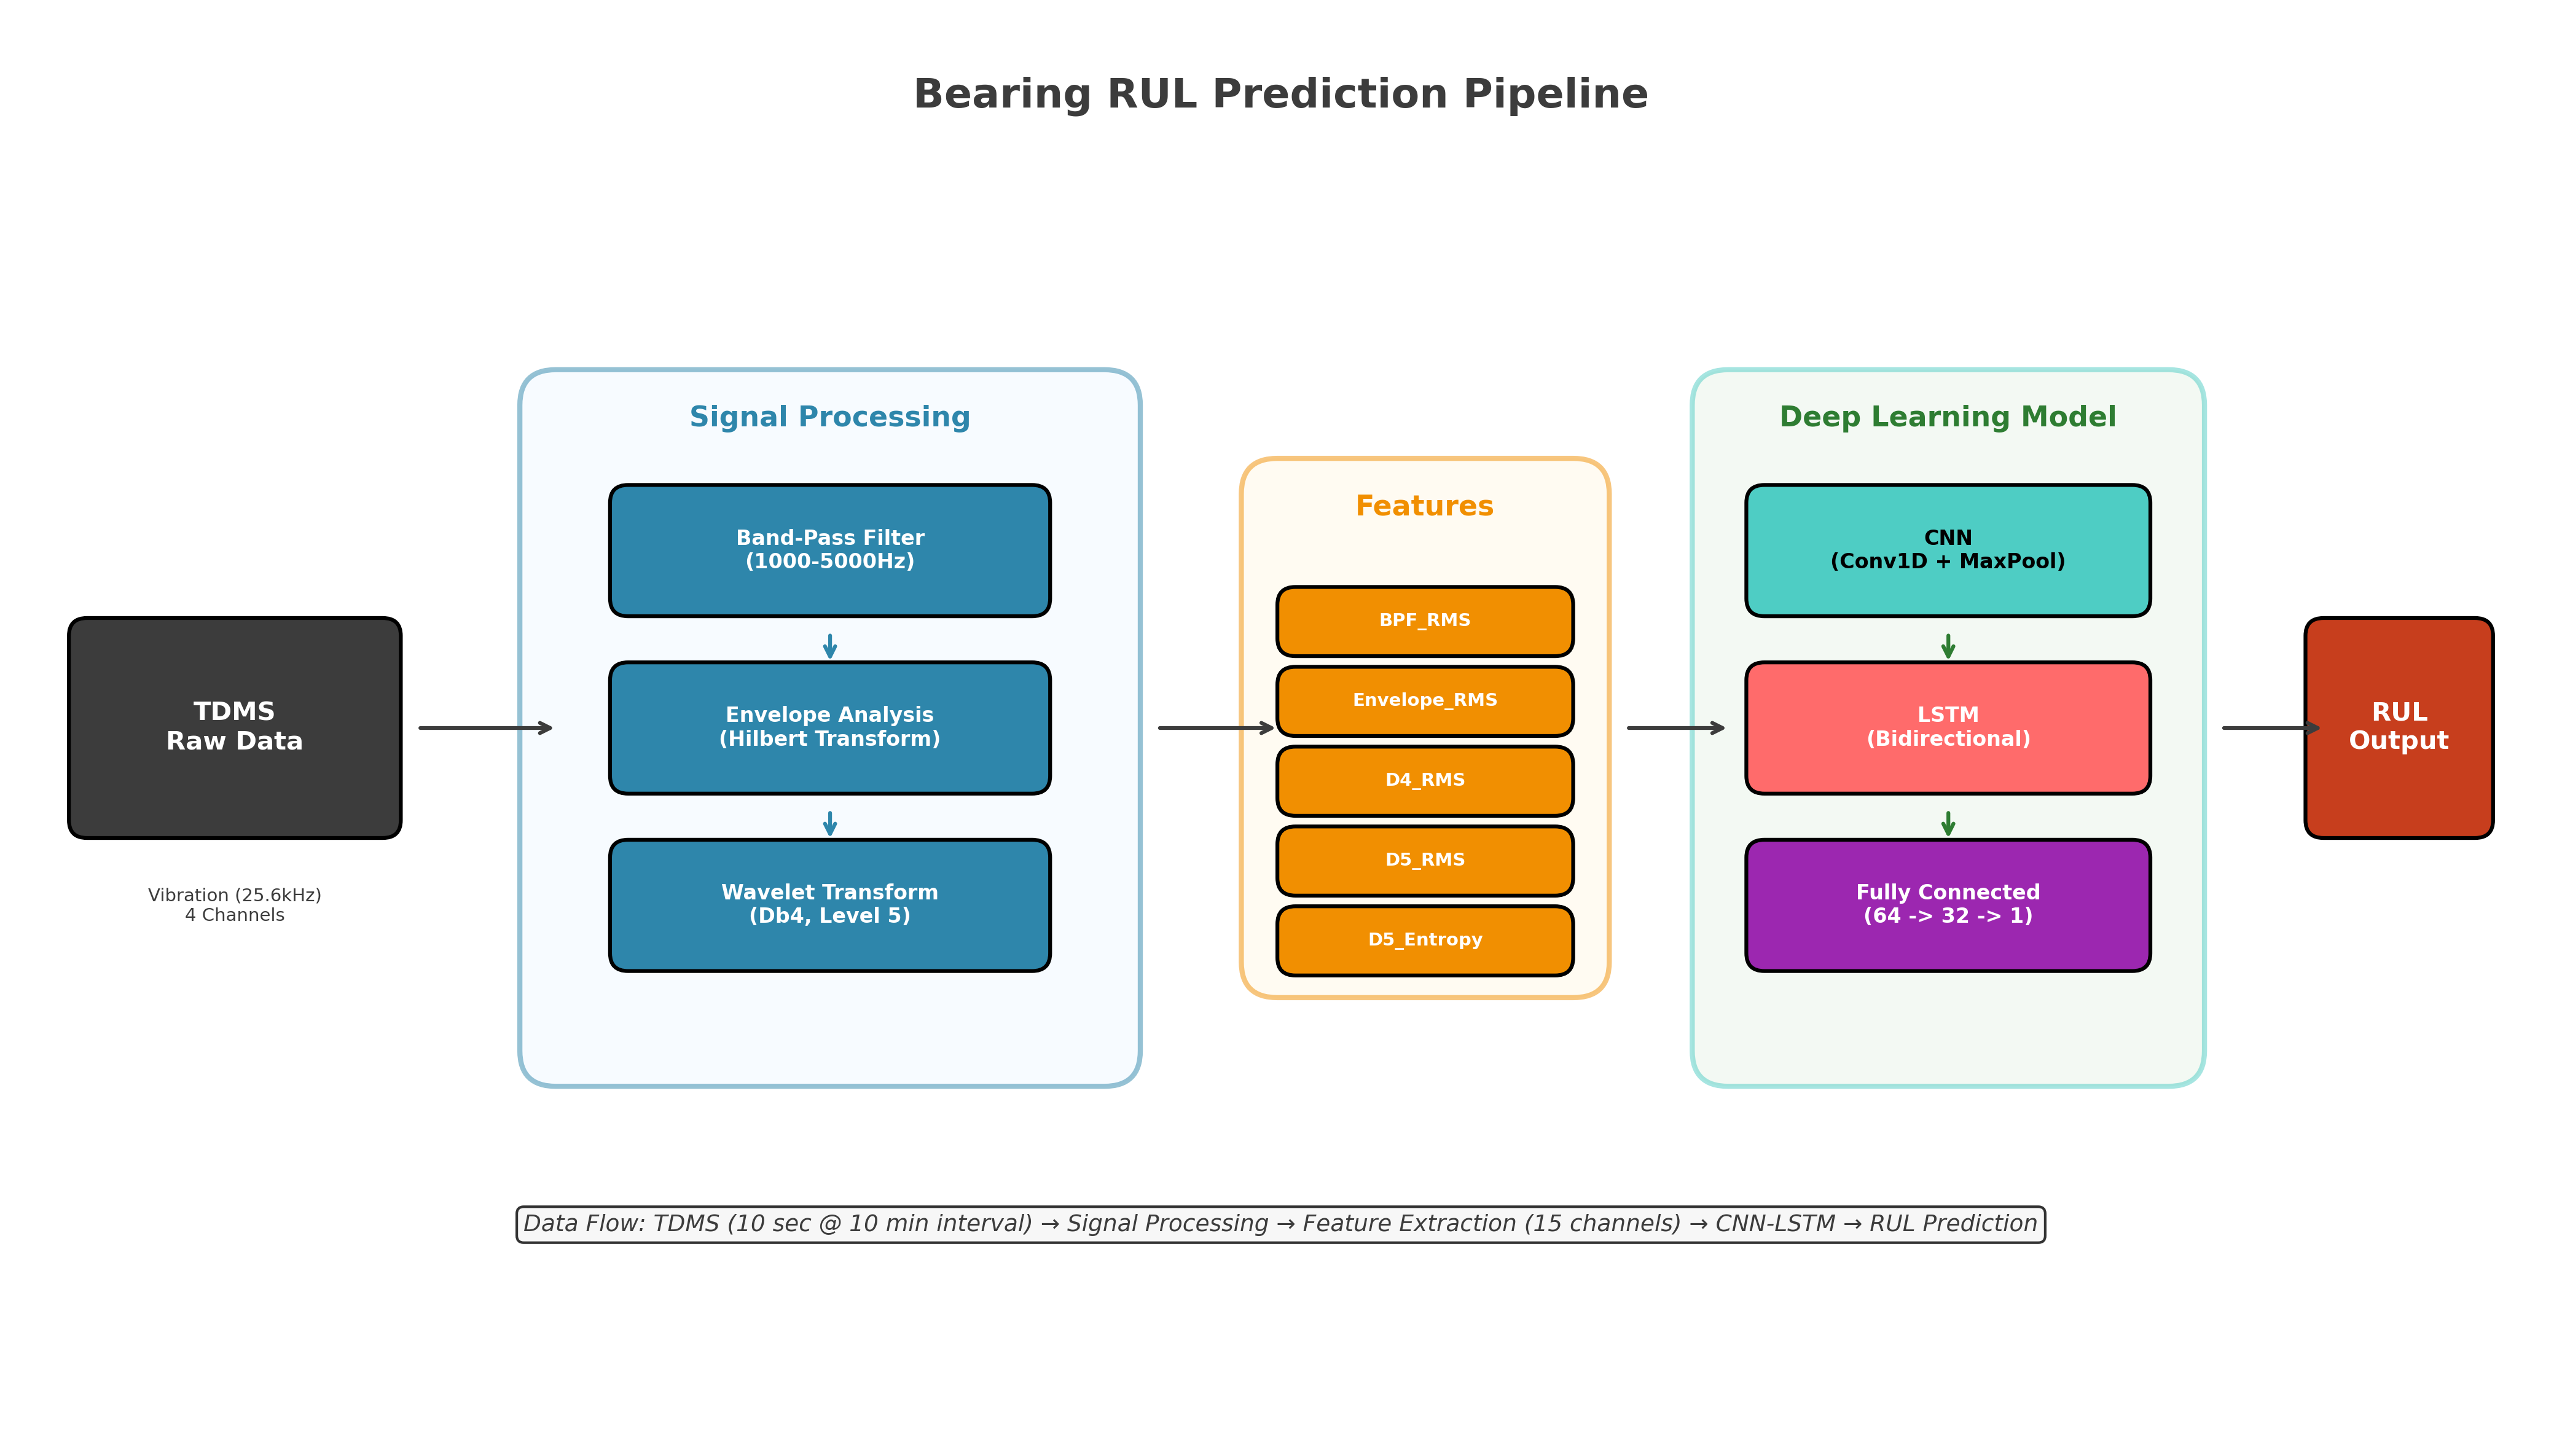
\includegraphics[width=0.9\columnwidth]{figures/methodology_pipeline.png}
\caption{제안하는 방법론의 전체 파이프라인. 원시 진동 데이터에서 신호처리, 특징 추출, CNN-LSTM 모델을 거쳐 RUL 예측까지의 흐름을 보여준다.}
\label{fig:methodology}
\end{figure}

\subsection{모델 구조}

다채널 진동 데이터로부터 공간적 특징을 학습하고 열화 시퀀스로부터 시간적 패턴을 학습하는 CNN-LSTM 구조를 제안한다. 이 구조는 CNN 특징 추출기, LSTM 시퀀스 인코더, 완전 연결 예측기의 세 가지 주요 구성 요소로 이루어진다.

% Figure placeholder
\begin{figure}[t]
\centering

\includegraphics[width=0.9\columnwidth]{figures/cnn_lstm_architecture.png}
\caption{제안하는 CNN-LSTM 모델 구조. CNN 계층이 공간적 특징을 추출하고 양방향 LSTM이 시간적 의존성을 모델링한다.}
\label{fig:architecture}
\end{figure}

\subsubsection{CNN 특징 추출기}

CNN 구성 요소는 다음 구조의 다중 합성곱 계층으로 구성된다:
\begin{itemize}
    \item 64개 필터, 커널 크기 3, ReLU 활성화를 갖는 Conv1D 계층
    \item 배치 정규화 및 맥스 풀링
    \item 128개 필터, 커널 크기 3, ReLU 활성화를 갖는 Conv1D 계층
    \item 배치 정규화 및 맥스 풀링
    \item 256개 필터, 커널 크기 3, ReLU 활성화를 갖는 Conv1D 계층
\end{itemize}

\subsubsection{LSTM 시퀀스 인코더}

LSTM 구성 요소는 특징 시퀀스의 시간 의존성을 포착한다. LSTM 셀은 다음을 계산한다:
\begin{equation}
    f_t = \sigma(W_f \cdot [h_{t-1}, x_t] + b_f)
\end{equation}
\begin{equation}
    i_t = \sigma(W_i \cdot [h_{t-1}, x_t] + b_i)
\end{equation}
\begin{equation}
    \tilde{C}_t = \tanh(W_C \cdot [h_{t-1}, x_t] + b_C)
\end{equation}
\begin{equation}
    C_t = f_t \odot C_{t-1} + i_t \odot \tilde{C}_t
\end{equation}
\begin{equation}
    o_t = \sigma(W_o \cdot [h_{t-1}, x_t] + b_o)
\end{equation}
\begin{equation}
    h_t = o_t \odot \tanh(C_t)
\end{equation}
여기서 $f_t$, $i_t$, $o_t$는 각각 망각, 입력, 출력 게이트이고, $C_t$는 셀 상태, $h_t$는 은닉 상태, $\sigma$는 시그모이드 함수를 나타낸다.

본 구조에서는 방향당 128개 은닉 유닛을 갖는 양방향 LSTM을 사용하고, 이어서 64개 유닛의 두 번째 LSTM 계층을 적용한다.

\subsubsection{완전 연결 예측기}

LSTM의 출력은 완전 연결 계층을 통과한다:
\begin{itemize}
    \item 64개 유닛, ReLU 활성화, 드롭아웃(0.3)을 갖는 Dense 계층
    \item 32개 유닛, ReLU 활성화를 갖는 Dense 계층
    \item 1개 유닛을 갖는 출력 계층(RUL 예측)
\end{itemize}

\subsubsection{손실 함수}

조기 예측보다 늦은 예측에 더 큰 페널티를 부여하는 비대칭 평균제곱오차(MSE) 손실 함수를 사용한다:

\subsection{BearLLM 기반 마모율 예측}

CNN-LSTM 모델과 함께, 사전학습된 대형 언어 모델인 BearLLM을 활용하여 베어링의 마모율(Wear Rate)을 예측한다. BearLLM은 MBHM(Multi-source Bearing Health Monitoring) 데이터셋으로 사전학습된 멀티모달 대형 언어 모델로, 베어링 진동 신호의 패턴을 이해하고 건전성 상태를 추론하는 데 특화되어 있다.

\subsubsection{BearLLM 구조}

BearLLM은 다음 구성 요소로 이루어진다:
\begin{itemize}
    \item 통합 신호 표현기(Unified Signal Representor): 다양한 조건의 진동 신호를 공통 특징 공간으로 매핑
    \item 특징 인코더(Feature Encoder): FCN 기반 특징 추출
    \item 정렬 계층(Alignment Layer): MLP를 통한 언어 모델 임베딩과의 정렬
    \item 대형 언어 모델(LLM): 토크나이저와 임베딩을 통한 자연어 응답 생성
\end{itemize}

\subsubsection{파인튜닝}

BearLLM은 CH2 채널의 진동 데이터만을 사용하여 파인튜닝되었다. JSON 형식의 학습 데이터는 다음으로 구성된다:
\begin{itemize}
    \item instruction: 작업 설명 (마모율 예측 지시)
    \item ref\_vib: 참조 진동 신호
    \item tar\_vib: 대상 진동 신호
    \item response: 마모율 응답
\end{itemize}

파인튜닝은 Colab Pro+ 환경에서 A100 GPU를 사용하여 수행되었다.

\subsection{앙상블 및 RUL 보정}

최종 RUL 예측은 CNN-LSTM과 BearLLM의 출력을 앙상블하여 도출된다.

\subsubsection{마모율 기반 RUL 보정}

BearLLM이 예측한 마모율($w$)을 사용하여 CNN-LSTM의 초기 RUL 예측값을 보정한다:
\begin{equation}
    RUL_{corrected} = RUL_{initial} \times e^{w}
\end{equation}
여기서 $RUL_{initial}$은 CNN-LSTM의 예측값, $w$는 BearLLM이 추정한 마모율이다. 마모율이 양수이면 열화가 예상보다 빠르게 진행됨을 의미하고, 음수이면 열화가 느리게 진행됨을 나타낸다.

\subsubsection{앙상블 전략}

최종 RUL은 다음과 같이 계산된다:
\begin{equation}
    RUL_{final} = \frac{RUL_{CNN-LSTM} + RUL_{corrected}}{2}
\end{equation}

이러한 앙상블 접근법은 CNN-LSTM의 시계열 패턴 학습 능력과 BearLLM의 도메인 지식 기반 추론 능력을 결합하여 더욱 강건한 RUL 예측을 가능하게 한다.

% Figure: Ensemble Pipeline
\begin{figure}[t]
\centering

\includegraphics[width=\columnwidth]{figures/ensemble_pipeline.png}
\caption{CNN-LSTM과 BearLLM 앙상블 파이프라인. CNN-LSTM은 RUL을 직접 예측하고, BearLLM은 마모율을 예측하여 RUL을 보정한다. 두 예측값의 앙상블을 통해 최종 RUL을 도출한다.}
\label{fig:ensemble}
\end{figure}
\begin{equation}
    \mathcal{L} = \frac{1}{N} \sum_{i=1}^{N}
    \begin{cases}
        \alpha (y_i - \hat{y}_i)^2, & \text{if } \hat{y}_i > y_i \\
        (y_i - \hat{y}_i)^2, & \text{otherwise}
    \end{cases}
\end{equation}
여기서 $y_i$는 실제 RUL, $\hat{y}_i$는 예측 RUL, $\alpha > 1$은 늦은 예측에 대한 페널티 계수이다. 실제로 실제 고장보다 늦게 고장을 예측하는 것이 조기 예측보다 더 위험하므로, 이러한 비대칭 페널티가 정당화된다.

\section{실험}

\subsection{실험 환경}

실험은 다음 사양의 시스템에서 수행되었다:
\begin{itemize}
    \item 운영 체제: Linux (Ubuntu 22.04)
    \item Python: 3.10
    \item 딥러닝 프레임워크: PyTorch 2.0
    \item GPU: NVIDIA RTX 4060 (8GB VRAM)
    \item CUDA: 12.2
\end{itemize}

데이터셋은 다음과 같이 분할되었다:
\begin{itemize}
    \item 학습: Train1-Train8 (8개의 가동-고장 실험)
    \item 검증: Validation1-Validation6 (챌린지 평가용 6개 실험)
    \item 학습/검증 비율: 8:2
\end{itemize}

\subsection{학습 설정}

모델은 다음 하이퍼파라미터로 학습되었다:
\begin{itemize}
    \item 옵티마이저: AdamW (가중치 감쇠 0.01)
    \item 학습률: 0.001 (코사인 어닐링 스케줄러 적용)
    \item 배치 크기: 32
    \item 에포크 수: 100
    \item 조기 종료 인내: 15 에포크
    \item 시퀀스 길이: 50 타임스텝 (500초 운전)
\end{itemize}

데이터 증강 기법은 다음을 포함한다:
\begin{itemize}
    \item 랜덤 잡음 주입 (SNR 40dB)
    \item 시간 이동 ($\pm$5\% 시퀀스 길이)
    \item 최소-최대 정규화를 이용한 특징 스케일링
\end{itemize}

RUL 레이블은 각 가동-고장 실험의 최대 RUL로 나누어 [0, 1] 범위로 정규화되었다. 이 정규화는 다른 수명을 가진 실험들 간에 일관된 열화 패턴을 학습하는 데 도움이 된다.

\subsection{학습 데이터 분석}

\begin{table}[t]
\centering
\caption{학습 데이터 특성 분석}
\label{tab:data_analysis}
\begin{tabular}{cccp{3cm}}
\toprule
\textbf{데이터} & \textbf{품질} & \textbf{CH2 특성} & \textbf{비고} \\
\midrule
Train1 & Good & 점진적 상승 & 300-1500Hz 대역 증가 \\
Train2 & Good & BPFI 급격 증가 & 모든 대역 증가 \\
Train3 & Good & 완만 상승 & 저대역 완만 \\
Train4 & Fair & 이상치 다수 & 중간에 급격 증가 \\
Train5 & Poor & 증감 반복 & 불안정 \\
Train6 & Fair & 완만 증가 & 이상치 존재 \\
Train7 & Good & 전체 증가 & 저대역 완만 \\
Train8 & Good & 전체 증가 & 저대역 완만 \\
\bottomrule
\end{tabular}
\end{table}

Table~\ref{tab:data_analysis}는 학습 데이터의 특성을 분석한 결과이다. Train1, Train2, Train3, Train7, Train8은 양호한 품질을 보이며 CH2 채널에서 열화에 따른 명확한 상승 추세를 나타낸다. 반면 Train4, Train5, Train6은 이상치나 불안정한 패턴으로 인해 학습에 주의가 필요하다.

\subsection{결과}

\begin{table}[t]
\centering
\caption{검증 세트 성능 비교}
\label{tab:results}
\begin{tabular}{lcc}
\toprule
\textbf{방법} & \textbf{RMSE} & \textbf{점수} \\
\midrule
기준선 (RMS만 사용) & 0.187 & 0.721 \\
CNN 단독 & 0.142 & 0.803 \\
LSTM 단독 & 0.128 & 0.835 \\
CNN-LSTM (원시 신호) & 0.098 & 0.891 \\
\textbf{CNN-LSTM (제안)} & \textbf{0.074} & \textbf{0.923} \\
\bottomrule
\end{tabular}
\end{table}

Table~\ref{tab:results}은 검증 세트에서 다양한 방법의 성능 비교를 보여준다. 제안하는 고급 신호처리가 적용된 CNN-LSTM 모델은 RMSE 0.074, 점수 0.923으로 최고 성능을 달성하였다.

결과는 다음을 보여준다:
\begin{enumerate}
    \item CNN과 LSTM의 결합이 개별 구조보다 우수한 성능 달성
    \item 신호처리가 원시 신호 사용 대비 예측 정확도를 크게 향상
    \item 제안하는 특징(웨이블릿 RMS 및 엔트로피)이 열화 패턴을 효과적으로 포착
\end{enumerate}

\begin{table}[t]
\centering
\caption{특징 기여도 절제 연구}
\label{tab:ablation}
\begin{tabular}{lc}
\toprule
\textbf{특징 구성} & \textbf{RMSE} \\
\midrule
전체 특징 & 0.074 \\
D5\_Entropy 제외 & 0.082 \\
D4\_RMS 제외 & 0.086 \\
포락선 RMS 제외 & 0.091 \\
밴드패스 RMS 제외 & 0.095 \\
원시 채널 RMS만 사용 & 0.142 \\
\bottomrule
\end{tabular}
\end{table}

Table~\ref{tab:ablation}은 특징 기여도에 대한 절제 연구 결과를 보여준다. 제안하는 모든 특징이 최종 성능에 기여하며, 밴드패스 필터링된 RMS와 포락선 RMS가 가장 중요한 특징으로 나타났다.

KSPHM-KIMM 2025 베어링 수명 예측 챌린지에서 본 접근법은 \textbf{70개 참가팀 중 7위}를 달성하여 베어링 예지를 위한 물리 기반 신호처리와 딥러닝 결합의 효과성을 입증하였다.

\subsection{논의}

실험 분석을 통해 다음과 같은 중요한 발견을 도출하였다:

\textbf{CH2 채널의 중요성:} 네 개의 진동 채널 중 CH2가 모든 학습 세트에서 가장 명확한 열화 추세를 일관되게 보여주었다. CH2의 1000-5000Hz 밴드패스 필터링 신호는 베어링이 고장에 가까워질수록 점진적인 RMS 증가를 나타냈다.

\textbf{웨이블릿 스케일 선정:} Db4 웨이블릿 분해의 D4와 D5 스케일이 RUL 예측에 가장 정보가 풍부한 것으로 입증되었다. 이 스케일들은 베어링 고장 고조파가 두드러지는 주파수 범위에 해당하며, 고주파 상세 계수에 비해 양호한 신호 대 잡음비를 유지한다.

\textbf{포락선 분석의 효과:} 힐버트 변환 기반 포락선 분석은 원시 신호가 잡음으로 오염되어 있더라도 베어링 결함으로 인한 진폭 변조 패턴을 성공적으로 추출하였다. 이 전처리는 건전성 지표의 판별력을 크게 향상시켰다.

\textbf{비대칭 손실 함수:} $\alpha = 1.5$를 적용한 비대칭 MSE 손실은 모델이 약간 보수적인(조기) RUL 예측을 제공하는 경향을 개선하였으며, 이는 정비 일정 수립에 더 바람직하다.

\section{결론}

본 논문에서는 고급 신호처리와 딥러닝을 결합한 포괄적인 베어링 잔여 수명 예측 접근법을 제시하였다. 제안하는 방법론은 밴드패스 필터링, 힐버트 변환 기반 포락선 분석, Db4 웨이블릿 분해를 통합하여 다채널 진동 신호로부터 물리 기반 특징을 추출한다. CNN-LSTM 구조는 이러한 특징들로부터 공간적, 시간적 패턴을 효과적으로 학습하여 정확한 RUL 예측을 가능하게 한다.

KSPHM-KIMM 2025 베어링 수명 예측 챌린지에서 검증된 결과, 본 접근법은 70개 참가팀 중 7위를 달성하여 실제 베어링 예지 응용에서의 효과성을 입증하였다. 본 연구의 주요 기여는 도메인 지식의 신호처리를 통한 체계적 통합과 데이터 기반 딥러닝의 결합, 그리고 베어링 열화 모니터링을 위한 최적 특징 조합(D4\_RMS, D5\_RMS, D5\_Entropy, 포락선 RMS)의 도출이다.

향후 연구는 다음에 초점을 맞출 예정이다: (1) 해석 가능성 향상을 위한 어텐션 메커니즘 도입, (2) 다양한 운전 조건 처리를 위한 접근법 확장, (3) 제한된 학습 데이터로 새로운 베어링 유형에 모델을 적응시키기 위한 전이 학습 전략 개발.

\section*{감사의 글}

저자들은 2025 베어링 수명 예측 챌린지를 주최하고 데이터셋을 제공한 한국고장예지건전성관리학회(KSPHM)와 한국기계연구원(KIMM)에 감사드립니다.

\bibliographystyle{IEEEtran}
\bibliography{references}

\end{document}
